\section{Rules of Probability}
Here we simply outline a few simple rules for probability that will help make the following discussion simpler to understand. Perhaps the simplest rule of probability is that given a series of possible outcomes, the sum of the probabilities of the outcome must equal unity. This is expressed as:
\begin{equation}\label{eqn:probsumdiscrete}
    \sum_{i=1}^{N} p_i = 1.
\end{equation}
Here $p_i$ represents the probability mass function, or more simply, the probability of the \textit{$i^{th}$} outcome, given $N$ possible events. If the random variable is continuous then we simply express this as an integral:
\begin{equation}\label{eqn:probsumcontinuous}
    \int p \left( x \right) dx = 1.
\end{equation}
Where $p(x)$ represents the probability density function of a particular outcome $x$.

Finally, we describe a few rules of adding probabilities, multiplying probabilities, and conditional probability. The probability of event A or event B, $P(A\textrm{ or }B)$ occurring is given as:
\begin{equation}
    P\left(A\textrm{ or }B\right) = P(A) + P(B) - P(A\textrm{ and }B).
\end{equation}
For which, the probability of two events occurring simultaneously is $P(A \textrm{ and } B)$:
\begin{equation}\label{eqn:probAandprobB}
    P\left(A\textrm{ and }B\right) \equiv P(A,B) = P(A) \, P(B|A) = P(B) \, P(A|B)
\end{equation}
This new term here $P(B|A)$ is to be interpreted as the probability that event B occurs given that A has occurred, and similarly, $P(A|B)$ means the probability that event A occurs given that B has occurred.

This last expression from Eq. \ref{eqn:probAandprobB} motivates the theorem known as Bayes Theorem, which we will express as follows:
\begin{equation} \label{eqn:BayesTheorem_basic}
     P(H|D) = \frac{P(H) \, P(D|H)}{P(D)}.
\end{equation}
In this formulation we have written, the probability of the hypothesis given the data, $P(H|D)$, is sometimes called the posterior probability. The probability of the hypothesis being true is $P(H)$, and is often called the prior probability. the probability of the data given the hypothesis, $P(D|H)$, which is called the likelihood. And finally we have the probability of obtaining the data, $P(D)$. We will devote a large amount of time in this work towards Bayes Theorem and its usefulness in conducting statistical inferences. 

\section{A Brief Introduction to Frequentist Statistics}
Frequentist statistics is the perspective that probabilities represent the frequency in which a random process will generate a particular result in the long-term. Frequentist statistics is a perspective that may be taken in the event that one expects to be able to examine the long term behavior of a particular random process. Furthermore, Frequentist statistical inference will place emphasis on the likelihood term, $P(D|H)$, from Eq. \ref{eqn:BayesTheorem_basic}. A choice on the probability of $P(H)$ is not made explicitly.

To better understand Frequentist statistics let us examine a toy problem. For example, consider an underlying random process that generates data, say 1 sample per second. Consider that this random process is described by a one-dimensional Gaussian distribution with zero-mean and unit-variance:
\begin{equation}\label{eqn:Gaussian}
    p(x) = \frac{1}{\sqrt{2\pi}} e^{\frac{-x^2}{2}}.
\end{equation}
This expression describes the probability density of obtaining some value of $x$ between $-\infty$ and $+\infty$. In particular, let's say that we are interested in making an inference on what probable values of $x$ as generated by this random process is. After recording data for 1 minute we would arrive at 60 samples, and so we only need record the frequency of values of $x$ that we obtain, binned in some appropriate way. Our posterior belief about plausible values of $x$ are purely informed by our measurements, i.e. the likelihood. We make no assumptions about the underlying random processor what the probability of obtaining some value of $x$ in the interval $-\infty$ and $+\infty$ is. Our understanding of the underlying distribution of $x$ is better informed when we collect more samples.

\subsection{Parameter Estimation and Confidence Intervals}
We will only briefly discuss parameter estimation and confidence intervals in the Frequentist regime since it is not widely used in this work. A more robust explanation of parameter estimation and confidence intervals can be found in Cousins et al.;

In the Frequentism we are interested in measuring some estimator of the underlying data. Ideally we would prefer that this estimator is unbiased, and has small variance so that we can gain confidence in our measurements. Frequentist confidence intervals are concerned with estimating what the width of the expected interval of variance of the estimator will be across multiple instances of sampling from the underlying data generating process.

The confidence interval is an inference made on the population parameters rather than on a particular sample set, which we will see is marked difference from Bayesian credible intervals.

\subsection{Null Hypothesis Significance Testing: Statistical Significance}
In Frequentist statistics we are often concerned with evaluating whether our particular data can be well-explained by a particular hypothesis. Notably, in science we are concerned whether the data we observe have a high probability of being generated by a null hypothesis, often that the data are not significantly different from what we might expect from noise processes alone.

The p-value represents the probability that the data (datum) is generated by the data-generating process in the null hypothesis. If we choose some confidence threshold  $\alpha$ that is sufficiently small, we can gain confidence in rejecting the null hypothesis if the p-value is smaller than this $\alpha$. This term $\alpha$ is sometimes called the significance level. Typically the p-value concerns the value of an estimator $x$ being greater (less) than some critical value, where the critical value is chosen so as to produce the right (left)-tailed probability $\alpha$. In the case of a right-tailed p-value we can write this in the following notation:
\begin{equation}\label{eqn:p_value}
    p(x \geq X | H_{0}) < \alpha.
\end{equation}
Typical choices of $\alpha$ are chosen to be small so as to (hopefully) reduce an incorrect rejection (or retention) of the null hypothesis $H_0$. One of the downsides of the p-value is that it states the probability of obtaining some value of $x$ given that the null hypothesis is true. This requires that the null hypothesis is a well-thought-out hypothesis and that it is an adequate model to test against in an experiment. In many areas of particle physics an $\alpha$ of $3 \times 10^{-7}$ is often chosen as an acceptable threshold to guard against false rejection of the null hypothesis. In general however, a choice of statistical significance threshold $\alpha$ is arbitrary.

\subsubsection{Controlling Error Rates}

In light of choosing a particular $\alpha$ threshold by which we choose to reject or retain the null hypothesis, we inevitably open ourselves up to error rates if we happen across a very improbable datum or data set that \textbf{is} generated by the null hypothesis.

Incorrect inferences in Frequentist statistical significance hypothesis testing are typically called \textit{Type I} (false positive) errors and \textit{Type II} (false negative) errors. Correct inferences are usually then called true positive inferences and true negative inferences. If the null hypothesis is true, and we set our significance threshold to $\alpha$, and we reject the null hypothesis, then we are making a false positive error. The probability of doing this is:
\begin{equation}
    p\left(\mathrm{rejecting \, H_{0}}| \mathrm{H_{0}} = \mathrm{True}\right) \equiv \alpha
\end{equation}
If we assume that the null hypothesis is true and choose $\alpha$ threshold for our p-value significance test, then the probability of failing to reject the null hypothesis when the null hypothesis is true is a true negative inference. The probability of doing this is:
\begin{equation}
    p\left(\mathrm{failing \, to \, reject \, H_{0}}| \mathrm{H_{0}} = \mathrm{True}\right) = 1 - \alpha
\end{equation}
 If we fail to reject the null hypothesis, but the null hypothesis is false, then we make a false negative error. We can ascribe the probability of doing this as:
 \begin{equation}
    p\left(\mathrm{rejecting \, H_{0}}| \mathrm{H_{0}} = \mathrm{False}\right) \equiv \beta
 \end{equation}
 The probability of rejecting the null hypothesis when the null hypothesis is false is given as:
 \begin{equation}
    p(\mathrm{failing \, to \, reject \, H_{0}}| H_{0} = \mathrm{False})= 1 - \beta    
 \end{equation}
 This probability, $1- \beta$ is sometimes called the \textit{power} of the statistical inference, since it tells us how efficacious the hypothesis test is in rejecting the null hypothesis when we should reject it (e.g. there is a gravitational wave present in the data and we find it). Hence we see that choosing an $\alpha$ level for rejecting the null hypothesis permits us to protect from Type I errors, false positives, and gives us some understanding on the probability of correctly assessing true negatives. However choosing an $\alpha$ level does not offer much in the way of protecting from Type II errors,  false negatives, nor much control over assessing true positives.

And so in the ideal situation of statistical significance evaluation in gravitational wave astronomy we want to get a handle for our inference on possible gravitational wave events. We thus introduce.


Finally, the last topic we describe is the problem of analyzing the data multiple times for statistical significance. This is sometimes called the problem of multiple comparisons or the look-elsewhere-effect. The problem can be simply explained under the following example. Say that one conducts a null-hypothesis statistical significance test at an $\alpha = 0.05$ threshold. . This opens the possibility of reporting a statistically significant result without properly attributing the number of trials conducted on the data. This is a form of misreporting in statistics and is sometimes called data-dredging or p-hacking. To correct for this possibility, a trials factor can be applied to a statistical significance test. One method for coherently assessing p-values after multiple comparisons is the Bonferroni correction wherein the $\alpha$ significance required to reject the null hypothesis is modified by the number of trials, $n$, performed. This can be expressed, to first order, as:
\begin{equation}
    p\left(\mathrm{rejecting \, H_{0} \, due \, to \, any \, trial}| \mathrm{H_{0}} = \mathrm{True}\right) = \frac{\alpha}{n}.
\end{equation}
Implicit in the Bonferroni correction is that each new search for the parameter of interest is independent of the other. This provides the most conservative case for correcting against false positives, but it opens the possibility of increasing the rate of false negatives. In practice, multiple comparisons are not always statistically independent and so other significance level adjustments for multiple comparisons are possible.

\section{A Brief Introduction to Bayesian Statistics}
Another interpretation of probability and statistical inference is Bayesian inference, which relies more heavily on all of the aspects of Eq. \ref{eqn:BayesTheorem_basic}. In Bayesianism, inference is performed by stating our assumptions at the outset of our experiment. We must outright state the probability distributions that we take as given in order for our inference to be complete. Probabilities here reflect our implicit ignorance or our level of belief in a particular hypothesis. We will describe in some detail the steps of statistical inference in Bayesian statistics below.

\subsection{Bayesian Inference}
Before conducting the experiment we need to start at the outset and describe our prior beliefs about plausible measurements that we could arrive at from our experiment. In general, there is no ``correct" method for assigning prior probabilities to the range of plausible measurements, however we provide some helpful guidelines below. Let us recall that the prior probability distribution must obey the standard rules of probability as outlined in Eqs. \ref{eqn:probsumdiscrete}, \ref{eqn:probsumcontinuous}.

In order to better illustrate choices of prior distribution let us consider the example for the data generating process, Eq. \ref{eqn:Gaussian} from the previous section.

The first prior distribution that we suggest is the uniform prior distribution. A uniform prior in $x$ would suggest that we assign a uniform probability to all possible values of $x$ possible. The expression for the probability density of a uniform continuous distribution in some interval, $b < x < a$ is given as:
\begin{equation}
    \pi(x, H) = \frac{1}{b - a}
\end{equation}
Here we have substituted the notation $P(H)$ for the prior distribution with $\pi(x, H)$, the probability distribution function of $x$ given this particular hypothesis choice, $H$. In this particular case our data generating procedure extends over all real values of $x$. Formally extending $pi$ to all values of $x$ would present a mathematical  problem. However, a reasonable choice of prior range can be chosen, such as $-10 < x < 10$, with, in this case, relatively little penalty.

The second prior distribution that we suggest is the informed prior distribution. Choosing an informed prior distribution is merely using our experimental expertise regarding the data generating procedure to provide a prior belief. Say for example, that the data generating procedure had been examined closely just prior to a recalibration of the machinery that generated the data. In a previous experiment, scientists estimated that the mean of a sample of the data was $0.12$, and with a variance of $1.02$. We might choose a prior distribution that used a Gaussian distribution with mean, $\mu = 0.12$, and variance, $\sigma^2 = 1.02$ for our inference. 

A third useful prior distribution to consider is a conjugate prior distribution. Conjugate prior distributions are sometimes available to certain kinds of likelihood distributions. If one has chosen a particular likelihood distribution and then the conjugate prior distribution to this likelihood distribution, then the posterior distribution will be in the same family of distributions as the conjugate prior distribution. This is advantageous if our prior beliefs on the family of the probability distribution that the data should belong to should not change with respect to the data. One example of a conjugate prior distribution is the Gamma distribution, when choosing a Poisson likelihood distribution. The posterior distribution is then proportional to another Gamma distribution.

There are many other methods of selecting a prior distribution function, of which we will discuss in further chapters.

Finally, after a prior distribution is chosen, the likelihood can be measured from the data and inference on the probability distribution of $x$ can be estimated as the product of the prior and the likelihood. This product is sometimes called the joint probability distribution and it is proportional to the posterior probability distribution function. The posterior probability distribution reflects our updated beliefs about plausible values of $x$.

Finally, the term $P(D)$ is sometimes called the evidence or the prior predictive. We will use the short hand, $\mathcal{E}$ for evidence from now on. It is called the evidence because its value represents the level of credibility we should assign our inference relative to other prior hypothesis choices. In a similar vein, the term prior predictive gives us an idea of how well of a job we did in predicting the data with our choice of prior. Lastly, we can compute the evidence by computing the marginal likelihood. Formally, this is done via,
\begin{equation}\label{eqn:marg_likelihood}
    \mathcal{E} = \int \pi(\vec{\theta}) \mathcal{L}(\vec{\theta}) d\vec{\theta},
\end{equation}
where we have used $\pi(\vec{\theta})$ for the prior distribution over all parameters $\vec{\theta}$, and likelihood distribution $\mathcal{L}(\vec{\theta})$. The marginal likelihood, or evidence, will be useful in Bayesian hypothesis testing. Many times the marginal likelihood is a difficult multi-dimensional integral to compute. Although oftentimes we are only interested in the marginal posterior probability distribution function for parameters, leading us to achieve adequate statistical inference without computing Eq. \ref{eqn:marg_likelihood}. Computation of the marginal likelihood is not often required for parameter estimation.

\subsection{Parameter Estimation and Credible Intervals}
Bayesian inference covers a method for performing parameter estimation of a particular data set. In particular, we aim to extract meaningful inference on the parameters of our data from the posterior distribution. This is in contrast to Frequentist statistical inference which only relies on the likelihood distribution for statistical inference.

To do so, first we introduce the concept of marginalization of the posterior probability distribution function. Marginalization of a probability distribution is the process of finding a probability distribution of a given parameter, $A$, by integrating the joint distribution of $A$ with the other parameters, over all the values of the other parameters. This approach is taken in finding the marginal likelihood in Eq. \ref{eqn:marg_likelihood}, however it can be done for any parameter of interest. Marginalization for a continuous probability distribution can be expressed as,
\begin{equation}
    p(x) = \int p(x|\vec{\theta}\,') \, p(\vec{\theta}\,') \, d\vec{\theta}\,',
\end{equation}
where the integration occurs over $d\vec{\theta}\,'$, all variables in the parameter set excluding $x$. This procedure is also known as integrating out \textit{nuisance parameters}, or can be thought of as the expectation value of the probability distribution of $x$ after averaging over all other parameters. This procedure of marginalization provides a useful and consistent method for estimating plausible parameter values for a data set.

It is often useful to summarize the results of our inference through summary statistics such as the mean, median, standard deviation, or interquartile range. One such method is to design a credible interval based around a mean, median value, a maximum likelihood estimate (\textit{MLE}), or a maximum marginal posterior probability (in \textit{Latin} this is \textit{maximum a posteriori}, hence it is usually termed the \textit{MAP}) estimate.

A credible interval can be designed by determining some confidence level $\alpha$ wherein we desire that $\alpha$ percent of the posterior probability distribution is contained between some surface or interval. For a 1-dimensional marginalized probability distribution, $\mathcal{P}(x)$ this takes the form:
\begin{equation}\label{eqn:credible_interval}
    \alpha = \int^{x_{high}}_{x_{low}} \mathcal{P}(x) dx.
\end{equation}
Thus, one can say that the random variable $x$ is believed to have an $\alpha$ percent probability of being between the interval $x_{low}$ and $x_{high}$. This procedure of credible intervals is not required to be 1-dimensional, and can pertain to credible surface contours. Choosing where to set $x_{low}$ and $x_{high}$ is somewhat subjective, although choosing the $10^{th}$ and $90^{th}$ percentiles of the posterior probability is common practice. This is called an equal-tailed interval, which we will use for the remainder of this work. Other examples of credible interval include the highest posterior density interval and choosing an interval that centers around the mean parameter values or MAP values 1995.

\subsection{Bayesian Hypothesis Testing}
\subsubsection{The Bayes Factor}
Another essential aspect of Bayesian inference is the evaluation of the statistical signficance of hypothesis choices. This occurs through evaluating the effectiveness of the choice in prior probability distribution. The marginal likelihood, $\mathcal{E}$, is the main driver behind establishing the level of evidence or support that the data has for a particular prior distribution choice. Simply put, the prior distribution that results in the largest evidence value is the model that has the most support.

Calculation of the odds for support of one hypothesis, $H_1$, over another hypothesis, $H_2$, is encapsulated in the following expression for the posterior odds ratio:
\begin{equation}\label{eqn:odds_ratio}
\mathcal{O}^{H_1\;\;}_{\;\;H_2} = \mathcal{B}^{H_1\;\;}_{\;\;H_2} \times \frac{\pi(H_1)}{\pi(H_2)}.
\end{equation}
In this equation, $\mathcal{O}^{H_1\;\;}_{\;\;H_2}$ represents the posterior odds that hypothesis $1$ is preferred over hypothesis $2$. The ratio of the evidences, $\mathcal{B}^{H_1\;\;}_{\;\;H_2} \equiv \frac{\mathcal{E}_{H_1}}{\mathcal{E}_{H_2}}$, between the two models is known as the Bayes factor. The Bayes factor provides an intuition for the relative support of one hypothesis over the other. The ratio $\frac{\pi(H_1)}{\pi(H_2)}$ represents our prior odds ratio, that is, how much more did we believe that hypothesis $1$ was preferred over hypothesis $2$ prior to our analysis. Said in another way, the prior odds ratio gives us a statement of what level of Bayes factor we would require before we begin to change our minds about the odds of hypothesis $2$ being better supported in the data than hypothesis $1$. When testing new physics, one may set the prior odds ratio to unity if one is fundamentally unsure about what hypotheses the data may support.

The posterior odds ratio then gives us a method for making a decision about whether to accept one hypothesis over the other hypothesis. One advantage to Bayesian hypothesis testing is that it gives us a straightforward method for testing hypotheses other than the null hypothesis that is commonly tested in Frequentist statistical inference. The downside however is that effectively and consistently computing Bayes factors remains an open area of research because of how difficult it can be to calculate the marginal likelihood. A conventional choice for hypothesis decision making is given to us by Jeffreys, and an alternative by Kass and Raftery 1995, see Fig. X.

An odds ratio can be converted into a probability of one hypothesis over another hypothesis through the following expression:
\begin{equation}\label{eqn:probability_odds_ratio}
    p^{H_1 \;\;}_{\;\;H_2} = \frac{\mathcal{O}^{H_1\;\;}_{\;\;H_2}}{1 + \mathcal{O}^{H_1\;\;}_{\;\;H_2}}.
\end{equation}
As such, a plot of the $\mathrm{log}_{10} \; \mathcal{O}^{H_1\;\;}_{\;\;H_2}$ can be made to suggest decision rules for odds ratios similar to choices on p-values in Frequentist statistics. As we can see in the plot below, when the odds ratio is 1 ($\mathrm{log}_{10} \; \mathcal{O} = 0$) the probability of one hypothesis versus another is $0.5$. 
\begin{figure}
  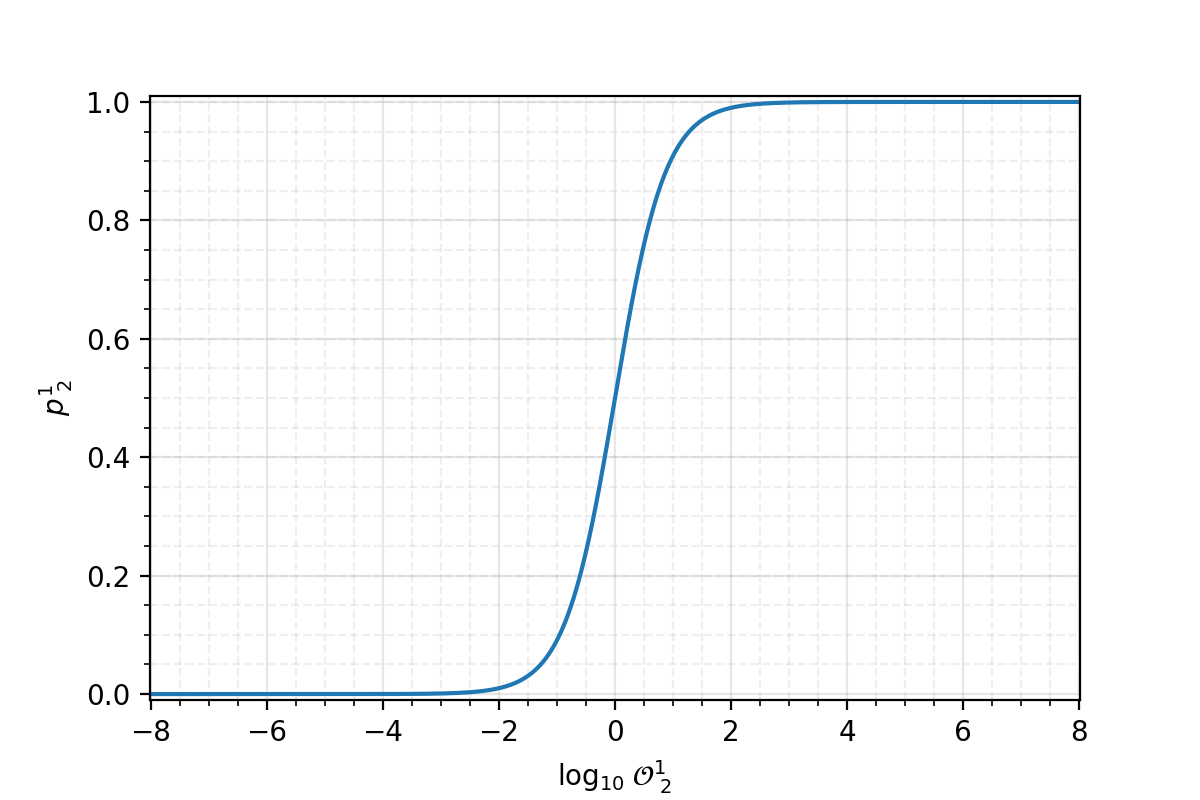
\includegraphics[width=\linewidth]{figs/chapter2/log10odds_probability.png}
  \caption{The probability of hypothesis 1 being favored over hypothesis 2 when considering the $\mathrm{log}_{10} \; \mathcal{O}$. When $\mathrm{log}_{10} \; \mathcal{O} = 0$, the probability for each hypothesis is $50\%$. At odds ratios close to 100 (0.01) the evidence becomes heavily stacked towards one hypothesis or another.}
  \label{fig:log10odds_v_probability}
\end{figure}
Furthermore, we can map this probability to a ranking statistic that is more familiar to Frequentists. That is the one-tailed z-score which states the integrated probability density from $-\infty$ to a particular multiple of the standard deviation of a Gaussian function. A z-score of $0 \sigma$ indicates a $50\%$ probability, while a z-score of $5 \sigma$ is $\sim$ $1-10^-7$ probability. We place a plot of this below for convenience.
\begin{figure}
  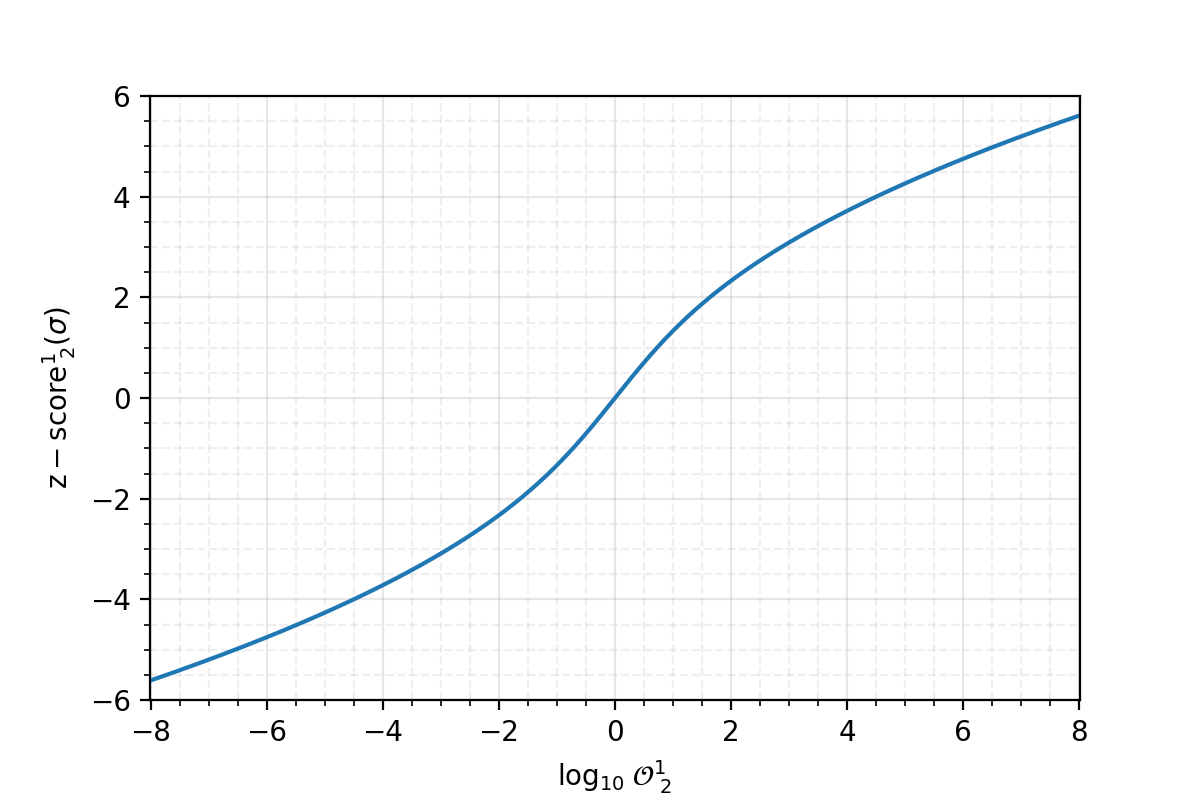
\includegraphics[width=\linewidth]{figs/chapter2/log10odds_z_score.png}
  \caption{The Frequentist z-score pertaining to the same level of probability for  hypothesis 1 being favored over hypothesis 2 when considering the $\mathrm{log}_{10} \; \mathcal{O}$. When $\mathrm{log}_{10} \; \mathcal{O} = 0$, the z-score is $0 \sigma$ and the probability for each hypothesis is $50\%$. A z-score of $>5 \sigma$ has the same probability value as an odds ratio of $> 10^7$.}
  \label{fig:log10odds_v_z_score}
\end{figure}

One convenient property of odds ratios is that we can stack evidence from multiple events if we continue to measure new data with our same prior hypotheses. In this manner, it is possible to take low significant results from multiple experiments and gradually build evidence for a hypothesis over many experiments. This requires that each experiment is a statistically independent event from the others, which is for all intents and purposes guaranteed in gravitational wave astronomy.

\subsubsection{Bayesian Model Averaging}

Bayesian statistics is based centrally around inferences from Bayes theorem. And as such there is no distinction necessary for inferences over parameters and inferences over models themselves. This provides a simple way to extend a singular analysis into an ongoing inference over multiple data sets or over multiple hypotheses. It provides a robust method for comparing and combining multiple inferences when data are informative or uninformative. As such we describe a methodology for combining the results of multiple hypothesis inferences called Bayesian model averaging as found in Kass and Raftery.

The concept of Bayesian model averaging is to average over many different models after evaluating the marginal likelihood for each model. In particular, one considers a fiducial standard model, $A$, of which the marginal likelihoood of $A$ will be compared to every other model. Thus for $N$ models we generate $N$ Bayes factors, where model $A$'s Bayes factor is simply unity since it is the fiducial standard model. In the case that all of the Bayes factors, $B_i$, are not definitive for one model or another, we must consider the possibility that since our parameters are conditioned on the model that we have elected, that we must seriously consider the effect of choice of model on various parameters. Given a sufficiently large set of models we can try to extract knowledge about the parameters that describe our data by marginalizing over many models. The formalism for this procedure follows immediately from Bayes theorem. Consider the following marginal posterior probability distribution for some model:
\begin{equation}
    \mathcal{P}(H_i|D) = \frac{\mathcal{B}^{H_i\;\;}_{\;\;H_A} \; \pi(H_i)}{\sum_{i=1}^N \mathcal{B}^{H_i\;\;}_{\;\;H_A} \; \pi(H_i)}.
\end{equation}
Here we have the posterior probability of some hypothesis given the data ... and the prior probability that we had for each model $H_i$...
Next, we consider a parameter $x$ that is present in all models thus considered such that our marginal posterior probability on $x$ given all of the models can become:
\begin{equation}
    \mathcal{P}(x|D) = \sum_{i=1}^N \mathcal{P}(x| D, H_i) \; \mathcal{P}(H_i|D).
\end{equation}
Here $\mathcal{P}(x| D, H_i)$ represents the marginal posterior probability distribution of $x$ under a particular hypothesis $H_i$, and so we coherently combine our inferences from multiple models by marginalizing over models. While, in practice there are an infinite number of models from which to draw inference on, there are usually only a finite set of probable models that we desire to investigate. All other models we can set our prior probabilities $\pi(H_i)$ to $0$, or sufficiently close to $0$ that they do not contribute to the analysis.

In the face of model uncertainty with respect to a particular data set, this provides us a consistent method for combining the results of multiple models in a self-consistent manner.

\subsubsection{Multiple Data Sets: Combining Evidence}
Multiplying through independent events...


Generally however, one must construct a model of models of sorts, a hyper-model that describes ...

\section{Frequentism and Bayesianism}
Above we have presented very brief outlines of different statistical frameworks which will be relevant to examining various hypotheses of gravitational wave analysis from aLIGO data. We have presented two statistical frameworks for examining hypotheses. The Frequentist interpretation is based on an interpretation of probability where if an outcome of some process is given a $70\%$ probability of occurring, this is to be interpreted that if the event is allowed to occur, under the same conditions, $100$ times, that we should expect the particular outcome to occur $70$ times. A Bayesian interpretation of probability is that we are trying to make a statement of our beliefs about how likely an outcome is to occur. Rather than probabilities describing the relative frequency that we can expect a particular result, probabilities encode our ignorance of the exact outcome of an event.

Both methods permit us to make rational inferences based on the measurements that we make in our data. Frequentist statistics has been a mainstay in gravitational wave astronomy for many years, but with the advent of advanced computational and numerical techniques, Bayesian statistics is seeing increasing use in gravitational wave astronomy.

While statistical inference give us some mathematical tools to better understand the correlations present in our data, they do not give us the full tools for making scientific decisions. The full expression of making a reasonable scientific inference relies in the experimental design and rational tools of investigation all the way through to conclusion. Statistics give us means to help justify some of these scientific choices but there is no statistical recourse for poor experimental design choices. It is always best to outline the research decisions made and try to account for plausible alternatives or future lines of investigation.
